\documentclass[11pt,a4paper]{article}
\usepackage[T1]{fontenc}
\usepackage[margin=2.3cm]{geometry}
\usepackage{amsmath,amssymb}
\usepackage{graphicx}
\usepackage[dvipsnames]{xcolor}
\usepackage{enumitem}
\usepackage[colorlinks=true,linkcolor=blue,urlcolor=blue]{hyperref}
\setlength{\parskip}{0.6em}
\setlength{\parindent}{0pt}
\begin{document}

\begin{center}{\LARGE\bfseries openfoundation}\\[0.4em]{\large Choose a footing size from the strength of the soil, in three sessions.}\\[0.2em]\small PAN IIT OSS explainer \textbullet{} diploma / undergraduate to advanced undergraduate (levels 5-6)\end{center}

\section*{Why this exists}
Every building stands on a foundation that spreads its weight into the ground. This explainer shows the mathematics behind that, from pressure under a footing to bearing capacity, settlement and consolidation, using only a few formulas and Python.

\section*{The end goal}
Choose a foundation size from soil bearing capacity. The end goal is to choose a foundation size from the soil bearing capacity and to understand how a change in soil strength changes the choice of foundation for a building. These are simplified teaching models and never a method for designing a real foundation.

\section*{How the three sessions build up}
\begin{enumerate}[nosep]
\item \textbf{Session 1: Spread the weight over enough ground} (Level 1, conceptual interactive model, 60 min).
\item \textbf{Session 2: From soil strength to footing size} (Level 2, mathematical engineering model, 75 min).
\item \textbf{Session 3: How far does it sink, and how fast?} (Level 3, simulation and validation, 90 min).
\end{enumerate}

\section{Session 1: Spread the weight over enough ground}

\subsection*{A. Real-world problem}
A stiletto heel can dent a wooden floor while an elephant does not, and a ten-storey building stands on soil that a heel would sink into. The force is large, so the builder spreads it over a wide footing under each column. If the footing is too small, the soil is overloaded and the building sinks or tilts. How wide must the footing be?

\subsection*{B. Concept and theory}
Pressure is force divided by the area it is spread over. With force in kilonewtons (kN) and area in square metres (m2), the pressure is in kilopascals (kPa); 1 kPa is 1 kN per m2. A column carrying load P sits on a square footing of side B, so the area is B times B and the pressure on the soil is P / B\textasciicircum{}2. Every soil can carry only so much pressure; the safe value is called the allowable bearing pressure q\_allow. Typical textbook ranges are soft clay about 50 to 100 kPa, firm clay 100 to 200 kPa and dense sand or gravel 200 to 400 kPa (rock is much higher). These ranges are only typical teaching values and must never be used for a real design. The footing is safe when P / B\textasciicircum{}2 is at most q\_allow, so the smallest side is B = sqrt(P / q\_allow). Doubling the side divides the pressure by four, because area grows with the square of the side.

\begin{itemize}[nosep]
\item P: column load (kN)
\item B: side of the square footing (m)
\item A: area of the footing, B times B (m2)
\item q: pressure on the soil, P / A (kPa)
\item q\_allow: allowable bearing pressure of the soil (kPa)
\end{itemize}

\begin{equation*}
q=\frac{P}{A}=\frac{P}{B^{2}}
\end{equation*}

\begin{equation*}
q\le q_{\mathrm{allow}}\quad\Longrightarrow\quad B\ge\sqrt{\frac{P}{q_{\mathrm{allow}}}}
\end{equation*}

\begin{equation*}
1\ \mathrm{kPa}=1\ \mathrm{kN/m^{2}}
\end{equation*}

\begin{center}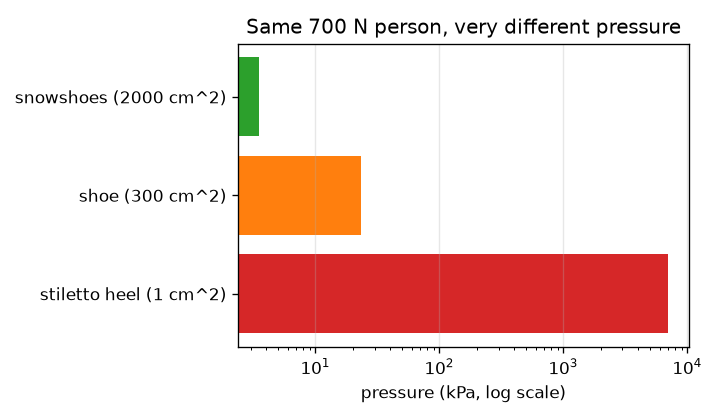
\includegraphics[width=0.85\linewidth]{figures/s01_heel_vs_snowshoe.png}\\\small The same 700 N person on a heel, a shoe and snowshoes (log scale).\end{center}

\subsection*{E. Worked example}
A 300 kN column stands on a 1.5 m square footing. Is that safe on soft clay with an allowable pressure of 75 kPa? If not, what is the smallest square footing, and what size would you build for a 100 kPa soil in 0.05 m steps?
\begin{enumerate}[nosep]
\item Area = 1.5 * 1.5 = 2.25 m2.
\item Pressure q = 300 / 2.25 = 133.3 kPa, which is more than 75 kPa: not safe.
\item Smallest side for 75 kPa: B = sqrt(300 / 75) = sqrt(4) = 2.0 m exactly (pressure 75 kPa, the boundary is allowed).
\item Sanity check: 2.0 m is wider than 1.5 m, as it must be for weaker soil.
\item For 100 kPa: B = sqrt(300 / 100) = 1.732 m, rounded up to 1.75 m (never round down).
\end{enumerate}
\textbf{Answer.} 1.5 m is not safe on 75 kPa soil (133.3 kPa). The smallest safe square footing is exactly 2.0 m; on 100 kPa soil build 1.75 m.

\subsection*{F. Questions}
\begin{enumerate}[nosep]
\item \textbf{Conceptual.} Why does a snowshoe stop you sinking even though your weight does not change? What does that say about a building?
\item \textbf{Numerical.} A 450 kN column stands on a 1.5 m square footing. Find the pressure, say whether it is safe on firm clay at 150 kPa, and find the smallest safe side.
\item \textbf{Graph and simulation interpretation.} On the pressure-against-width graph for a 300 kN column, what happens to the pressure when the width is halved? Where does the curve cross a 100 kPa soil line?
\item \textbf{Design and optimisation challenge.} Design: a 300 kN column could stand on soft clay (75 kPa) or on dense sand (300 kPa). Find the smallest square footing for each and compare the concrete area. What other things would an engineer worry about?
\end{enumerate}

\section{Session 2: From soil strength to footing size}

\subsection*{A. Real-world problem}
A 600 kN column must stand on soil whose allowable bearing pressure is 150 kPa. The concrete footing itself weighs something, so it presses on the soil too. And where does the allowable pressure come from? Engineers take the pressure at which the soil would fail and divide by a factor of safety. How wide must the footing be, and what if the load is not exactly in the middle?

\subsection*{B. Concept and theory}
The soil carries the column load P plus the footing weight 24 B\textasciicircum{}2 t (concrete is about 24 kN/m3, t is the footing thickness), so the contact pressure is q = P / B\textasciicircum{}2 + 24 t. Requiring q at most q\_allow gives B = sqrt(P / (q\_allow - 24 t)), rounded up. The allowable pressure comes from the ultimate bearing capacity q\_ult, the pressure at which the soil shears. Terzaghi's equation for a long strip footing is q\_ult = c N\_c + q N\_q + 0.5 gamma B N\_gamma, with c the soil cohesion (kPa), q = gamma D\_f the soil pressure beside the footing at its base, gamma the soil unit weight, B the width and N\_c, N\_q, N\_gamma bearing capacity factors that grow with the soil friction angle phi. For saturated clay loaded quickly (phi = 0) the factors are N\_c = 5.7, N\_q = 1 and N\_gamma = 0, so q\_ult = 5.7 c + gamma D\_f. The allowable pressure is q\_ult divided by a factor of safety FS, commonly about 3. For phi above zero the lesson computes N\_q and N\_c from Terzaghi's formulas; N\_gamma needs a table and is not computed here. If the load acts a distance e from the centre of a footing of width B and length L, the edge pressures are P / (B L) times (1 plus or minus 6 e / B). The smaller one reaches zero at e = B / 6 (the middle-third rule): beyond that the soil would have to pull on the footing, so the base lifts off, the contact length is 3 (B / 2 - e) and the largest pressure is 2 P / (3 L (B / 2 - e)).

\begin{itemize}[nosep]
\item P: column load (kN)
\item B, L: footing width and length (m)
\item t: footing thickness (m)
\item q: contact pressure on the soil (kPa)
\item c: soil cohesion (kPa)
\item gamma: soil unit weight (kN/m3)
\item D\_f: depth of the footing base (m)
\item N\_c, N\_q, N\_gamma: Terzaghi bearing capacity factors (no unit)
\item FS: factor of safety (no unit)
\item e: eccentricity of the load from the footing centre (m)
\end{itemize}

\begin{equation*}
q=\frac{P}{B^{2}}+\gamma_{c}\,t,\qquad B\ge\sqrt{\frac{P}{q_{\mathrm{allow}}-\gamma_{c}\,t}}
\end{equation*}

\begin{equation*}
q_{\mathrm{ult}}=cN_{c}+qN_{q}+\tfrac{1}{2}\gamma BN_{\gamma}
\end{equation*}

\begin{equation*}
\varphi=0:\quad q_{\mathrm{ult}}=5.7\,c+\gamma D_{f},\qquad q_{\mathrm{allow}}=\frac{q_{\mathrm{ult}}}{FS}
\end{equation*}

\begin{equation*}
q_{\max,\min}=\frac{P}{BL}\left(1\pm\frac{6e}{B}\right),\qquad e\le\frac{B}{6}\ \text{for no tension}
\end{equation*}

\begin{equation*}
e>\frac{B}{6}:\quad q_{\max}=\frac{2P}{3L\,(B/2-e)}
\end{equation*}

\begin{center}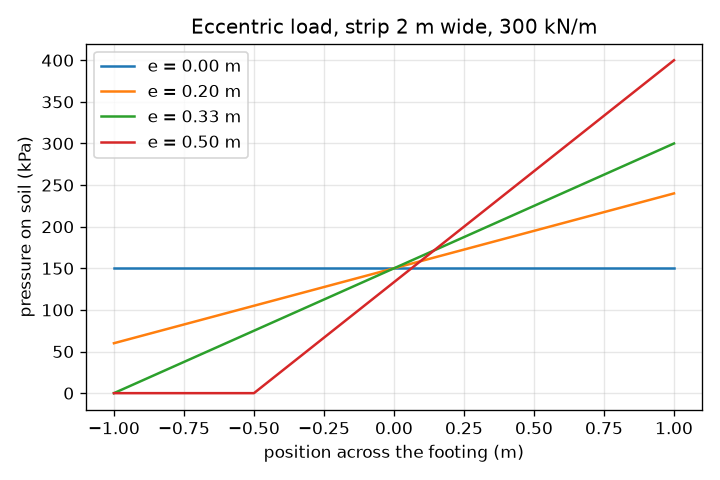
\includegraphics[width=0.85\linewidth]{figures/s02_eccentric_pressure.png}\\\small Pressure across a 2 m strip under 300 kN/m for four eccentricities.\end{center}

\subsection*{E. Worked example}
Design a square footing for a 600 kN column on soil with allowable pressure 150 kPa, thickness 0.6 m, built in 0.05 m steps. Then find the allowable pressure of a strip footing on clay with c = 50 kPa and FS = 3, and the edge pressures of a 2 m wide strip carrying 300 kN/m with e = 0.2 m.
\begin{enumerate}[nosep]
\item Footing weight per m2 = 24 * 0.6 = 14.4 kPa. The column may use 150 - 14.4 = 135.6 kPa.
\item B = sqrt(600 / 135.6) = 2.104 m, rounded up to 2.15 m. Check: q = 600 / 2.15\textasciicircum{}2 + 14.4 = 144.2 kPa, below 150. At 2.10 m the pressure would be 150.5 kPa, just too much.
\item Terzaghi, phi = 0: q\_ult = 5.7 * 50 = 285 kPa. With FS = 3, q\_allow = 285 / 3 = 95 kPa.
\item Eccentric strip: mean pressure = 300 / 2 = 150 kPa; 6 e / B = 6 * 0.2 / 2 = 0.6, so q\_max = 150 * 1.6 = 240 kPa and q\_min = 150 * 0.4 = 60 kPa. Since e = 0.2 m is below B / 6 = 0.333 m, there is no tension.
\end{enumerate}
\textbf{Answer.} Build a 2.15 m square footing (144.2 kPa). The allowable pressure on the c = 50 kPa clay is 95 kPa. The strip's edge pressures are 240 kPa and 60 kPa.

\subsection*{F. Questions}
\begin{enumerate}[nosep]
\item \textbf{Conceptual.} Why must the eccentricity stay within the middle third (e at most B / 6) for a footing on soil? What happens if it does not?
\item \textbf{Numerical.} A strip footing carries 200 kN/m on clay with c = 50 kPa. Using phi = 0, a factor of safety of 3 and ignoring the footing weight, what width is needed? Give the width you would build in 0.05 m steps.
\item \textbf{Graph and simulation interpretation.} From the required-width graph, what happens to the footing side for a 600 kN column when the allowable pressure falls from 150 kPa to 75 kPa? Compute it.
\item \textbf{Design and optimisation challenge.} Design: the 600 kN column in the worked example also carries a moment that makes the load act 0.2 m off-centre in a square footing (t = 0.6 m, 150 kPa allowable including the footing weight). Find the smallest side in 0.05 m steps with e at most B / 6 and a peak pressure no greater than 150 kPa. How much more plan area does the eccentricity cost?
\end{enumerate}

\section{Session 3: How far does it sink, and how fast?}

\subsection*{A. Real-world problem}
A footing can be strong enough and still sink too far, or sink more under one column than under its neighbour, which cracks walls. Settlement has two parts: an immediate elastic part, and in clay a slow squeezing-out of water called consolidation that can take years. How much will a 600 kN column sink, how long will it take, and how do you size the footings of a building so that it settles evenly?

\subsection*{B. Concept and theory}
Elastic settlement. Treat the soil as an elastic half-space with Young's modulus E and Poisson's ratio nu. A footing of width B carrying pressure q settles s = q B (1 - nu\textasciicircum{}2) I / E, where I is an influence factor depending on shape and stiffness. We choose I = 0.82 for a rigid square footing (a textbook value); the checkpoint brackets it between the rigid circle (pi / 4 = 0.785) and the average of a uniformly loaded flexible square (about 0.95, centre 1.122). For the same pressure a wider footing settles more; for the same load a wider footing settles less, s = k P / B. Consolidation. A saturated clay layer of thickness H, compression index Cc, initial void ratio e0 and initial effective stress sigma0 (at mid-layer) squeezes under an added stress dsigma by s = H Cc / (1 + e0) log10((sigma0 + dsigma) / sigma0). Terzaghi's theory gives the time: the time factor T\_v = c\_v t / H\_dr\textasciicircum{}2 (c\_v coefficient of consolidation, H\_dr the longest drainage path) and the average degree of consolidation U = 1 - sum of 2 / M\textasciicircum{}2 exp(-M\textasciicircum{}2 T\_v) with M = (2m + 1) pi / 2. It gives U = 50 percent at T\_v = 0.197 and U = 90 percent at T\_v = 0.848. Stress with depth. The 2:1 rule (an approximation) spreads the load at 2 vertical to 1 horizontal, so a square footing P of side B gives P / (B + z)\textasciicircum{}2 at depth z. Boussinesq's elastic solution for a point load gives 3 P / (2 pi z\textasciicircum{}2) on its axis, and in general 3 P z\textasciicircum{}3 / (2 pi R\textasciicircum{}5); summing it over the footing area gives the stress under a real footing. Failure cases are bearing failure (pressure above q\_ult / FS) and differential settlement between neighbouring columns.

\begin{itemize}[nosep]
\item q: pressure on the soil (kPa)
\item B: footing width (m)
\item E, nu: Young's modulus and Poisson's ratio of the soil (kPa, no unit)
\item I: influence factor (0.82 chosen for a rigid square footing) (no unit)
\item H, Cc, e0: clay thickness, compression index, initial void ratio (m, no unit, no unit)
\item sigma0, dsigma: initial effective stress and added stress at mid-layer (kPa)
\item c\_v, H\_dr, t: coefficient of consolidation, drainage path, time (m2/year, m, year)
\item T\_v, U: time factor and average degree of consolidation (no unit)
\item z, P: depth below the footing and load (m, kN)
\end{itemize}

\begin{equation*}
s=\frac{q\,B\,(1-\nu^{2})\,I}{E}
\end{equation*}

\begin{equation*}
s_{c}=\frac{H\,C_{c}}{1+e_{0}}\log_{10}\frac{\sigma_{0}+\Delta\sigma}{\sigma_{0}}
\end{equation*}

\begin{equation*}
T_{v}=\frac{c_{v}\,t}{H_{dr}^{2}},\qquad U=1-\sum_{m=0}^{\infty}\frac{2}{M^{2}}e^{-M^{2}T_{v}},\quad M=\frac{(2m+1)\pi}{2}
\end{equation*}

\begin{equation*}
\Delta\sigma_{2:1}=\frac{P}{(B+z)^{2}},\qquad \Delta\sigma_{z}=\frac{3P}{2\pi z^{2}}\ \text{(point load, on the axis)}
\end{equation*}

\begin{equation*}
\Delta\sigma_{z}=\frac{3Pz^{3}}{2\pi R^{5}},\qquad R^{2}=x^{2}+y^{2}+z^{2}
\end{equation*}

\begin{center}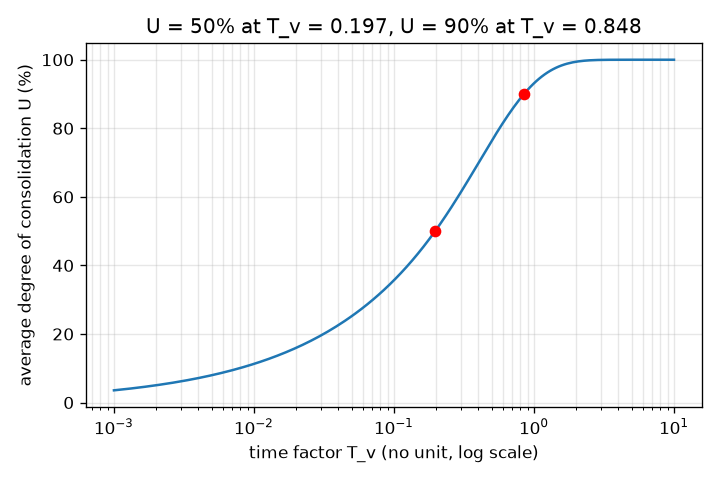
\includegraphics[width=0.85\linewidth]{figures/s03_consolidation_curve.png}\\\small Average degree of consolidation against time factor: 50 percent at 0.197, 90 percent at 0.848.\end{center}

\subsection*{E. Worked example}
A 2 m square rigid footing carries 150 kPa on soil with E = 20 MPa and nu = 0.3. Below it a 4 m clay layer (Cc 0.3, e0 0.9) has sigma0 = 100 kPa and dsigma = 50 kPa at mid-layer, c\_v = 1.5 m2/year and drains at top and bottom (H\_dr = 2 m). Find the elastic settlement, the consolidation settlement, the total, and the times for 50 and 90 percent consolidation.
\begin{enumerate}[nosep]
\item Elastic: s = 150 * 2 * (1 - 0.3\textasciicircum{}2) * 0.82 / 20000 = 150 * 2 * 0.91 * 0.82 / 20000 = 0.0112 m = 11.2 mm.
\item Consolidation: s\_c = 4 * 0.3 / 1.9 * log10(150 / 100) = 0.6316 * 0.1761 = 0.1112 m = 111.2 mm.
\item Total = 11.2 + 111.2 = 122.4 mm.
\item Time: t = T\_v H\_dr\textasciicircum{}2 / c\_v. For 50 percent, T\_v = 0.197: t50 = 0.197 * 4 / 1.5 = 0.52 years.
\item For 90 percent, T\_v = 0.848: t90 = 0.848 * 4 / 1.5 = 2.26 years. Doubling the drainage path would make this 4 times longer.
\end{enumerate}
\textbf{Answer.} Elastic 11.2 mm, consolidation 111.2 mm, total 122.4 mm; 50 percent of the consolidation takes 0.52 years and 90 percent takes 2.26 years.

\subsection*{F. Questions}
\begin{enumerate}[nosep]
\item \textbf{Conceptual.} Why does consolidation take years in clay, and why does halving the drainage path make it much faster?
\item \textbf{Numerical.} A clay layer 3 m thick (Cc 0.3, e0 0.9) has sigma0 = 100 kPa and dsigma = 50 kPa at mid-layer. Find the final consolidation settlement.
\item \textbf{Graph and simulation interpretation.} On the consolidation curve with c\_v = 1.5 m2/year and H\_dr = 2 m, at what times are 50 and 90 percent of the settlement reached?
\item \textbf{Design and optimisation challenge.} Design: two columns carry 250 kN and 1200 kN. The bearing-only footings are 1.40 m and 3.00 m (settlements 6.7 and 14.9 mm). With E = 20 MPa and nu = 0.3, find the smallest width for the big footing in 0.05 m steps so that the two settlements differ by at most 3.5 mm. What does it cost?
\end{enumerate}

\section{Real-world mini-project}
\textbf{Even settlement for a small building (classroom exercise only).} A small building has four columns carrying 250, 450, 800 and 1200 kN on soil with an allowable pressure of 150 kPa and an elastic modulus E = 20 MPa (Poisson ratio 0.3, footing thickness 0.6 m, rigid square footings with I = 0.82). If each footing is sized only for bearing, the settlements differ by 8.26 mm, which can crack walls. Use \texttt{design\_for\_target} and \texttt{settlements} from Session 3 and scan target settlements from 6.0 mm to 20.0 mm in steps of 0.5 mm. Your classroom limit is a differential settlement of at most 4 mm. Find the target with the smallest total footing plan area that meets the limit. This is a teaching exercise: real design also needs the footing interaction, consolidation, groundwater, structural stiffness and a qualified engineer.

\section{The path ahead}
\begin{enumerate}[nosep]
\item \textbf{Session 4: Neighbouring footings and overlapping bulbs.} A function giving the added vertical stress at any point (x, y, z) from several rectangular footings.
\item \textbf{Session 5: Staged loading in time.} A settlement-time function for a load applied half at time zero and half after one year.
\item \textbf{Session 6: A combined footing for two columns.} A search over the width of a 4 m long footing carrying 600 kN and 300 kN columns 3 m apart, each 0.5 m from the nearest end.
\item \textbf{Session 7: Uncertain soil strength.} A Monte Carlo run of 200000 samples of a lognormal cohesion with mean 50 kPa and 30 percent coefficient of variation under a strip footing pressure of 114.4 kPa.
\end{enumerate}

\section{Answers and hints}

\subsection*{Session 1}
\begin{enumerate}[nosep]
\item \textbf{Conceptual.} Hint: Compare the areas, and think about what soil responds to. Solution: Soil responds to pressure, force per area, not to force alone. A snowshoe spreads the same weight over a much larger area, so the pressure is far smaller (3.5 kPa against 7000 kPa for a stiletto heel in the model). A building does the same with footings: it spreads each column load over enough ground that the pressure stays below what the soil can carry.
\item \textbf{Numerical.} Hint: Area = B\textasciicircum{}2, then q = P / A. The smallest side is sqrt(P / q\_allow). Solution: q = 450 / 2.25 = 200 kPa, which is above 150 kPa: not safe. Smallest side = sqrt(450 / 150) = sqrt(3) = 1.732 m, so build 1.75 m. Check: 450 / 1.75\textasciicircum{}2 = 147 kPa, below 150.
\item \textbf{Graph and simulation interpretation.} Hint: Pressure goes as 1 / B\textasciicircum{}2. Solve 300 / B\textasciicircum{}2 = 100. Solution: Halving the width makes the area four times smaller, so the pressure becomes four times larger. The curve crosses the 100 kPa line at B = sqrt(300 / 100) = 1.73 m; wider footings are safe, narrower ones are not.
\item \textbf{Design and optimisation challenge.} Hint: Use B = sqrt(P / q\_allow) for each soil and compare B\textasciicircum{}2. Solution: Soft clay: B = sqrt(300 / 75) = 2.0 m, area 4.0 m2. Dense sand: B = sqrt(300 / 300) = 1.0 m, area 1.0 m2. The footing on clay needs four times the plan area. Trade-off: a wider footing costs more concrete and excavation; an engineer must also check settlement (Session 3), the footing's own weight, groundwater, depth of frost and loads that act off-centre. This model is for teaching only.
\end{enumerate}

\subsection*{Session 2}
\begin{enumerate}[nosep]
\item \textbf{Conceptual.} Hint: Can soil pull on a footing? Look at the smaller edge pressure. Solution: The smaller edge pressure is P / (B L) times (1 - 6 e / B), which reaches zero at e = B / 6. Soil cannot pull on the footing, so beyond that the base lifts off on one side: the contact area shrinks and the largest pressure rises sharply (400 kPa instead of 240 kPa in our example with e = 0.5 m for a 2 m strip), and the footing may tilt.
\item \textbf{Numerical.} Hint: q\_ult = 5.7 c, q\_allow = q\_ult / 3, then B = load per metre / q\_allow. Solution: q\_ult = 5.7 * 50 = 285 kPa; q\_allow = 95 kPa; B = 200 / 95 = 2.105 m, so build 2.15 m. Check: 200 / 2.15 = 93 kPa, below 95 kPa.
\item \textbf{Graph and simulation interpretation.} Hint: B = sqrt(600 / (q\_allow - 14.4)), then round up. Solution: At 150 kPa the side is 2.15 m; at 75 kPa it is sqrt(600 / 60.6) = 3.15 m (rounded up to 3.15 m). Halving the soil strength increases the width by about 46 percent and the area by more than double, because the curve is steep at the weak-soil end.
\item \textbf{Design and optimisation challenge.} Hint: Peak pressure = P / B\textasciicircum{}2 * (1 + 6 e / B) + 14.4. Try sides from 2.15 m upward. Solution: Try B = 2.55 m: peak = 600 / 6.5025 * (1 + 1.2 / 2.55) + 14.4 = 150.1 kPa, slightly too high. B = 2.6 m: peak = 144.1 kPa, safe, and e = 0.2 m is below B / 6 = 0.43 m. The plan area is 2.6\textasciicircum{}2 = 6.76 m2 against 2.15\textasciicircum{}2 = 4.62 m2: about 46 percent more concrete. Trade-off: reduce the moment (stiffer connection, tie beams) or accept a bigger footing.
\end{enumerate}

\subsection*{Session 3}
\begin{enumerate}[nosep]
\item \textbf{Conceptual.} Hint: Water must flow through very small pores. Look at H\_dr in T\_v. Solution: The load is first carried by the water in the pores; the settlement happens only as that water flows out through tiny pores, which clay allows very slowly (small c\_v). Time is proportional to H\_dr\textasciicircum{}2, so halving the drainage path makes consolidation four times faster (a doubled path makes it four times slower).
\item \textbf{Numerical.} Hint: s = H Cc / (1 + e0) log10((sigma0 + dsigma) / sigma0). Solution: s = 3 * 0.3 / 1.9 * log10(1.5) = 0.4737 * 0.1761 = 0.0834 m = 83.4 mm. Sanity check: 3/4 of the 4 m layer's 111.2 mm = 83.4 mm, as it must be since settlement is proportional to the thickness.
\item \textbf{Graph and simulation interpretation.} Hint: t = T\_v H\_dr\textasciicircum{}2 / c\_v with T\_v = 0.197 and 0.848. Solution: t50 = 0.197 * 4 / 1.5 = 0.52 years and t90 = 0.848 * 4 / 1.5 = 2.26 years. The curve is steep early (half the settlement in about 6 months) and then flattens, so the last 10 percent takes far longer than the first 50.
\item \textbf{Design and optimisation challenge.} Hint: s = k P / B with k = 0.91 * 0.82 / 20000. The big footing may settle at most 3.5 mm more than the small one. Solution: The small footing settles 6.66 mm. The big one may settle up to 10.16 mm: B \textgreater{}= k * 1200 / 0.0101625 = 4.406 m, so build 4.45 m (settlement 10.06 mm, difference 3.4 mm; 4.40 m would give 3.51 mm, just too much). Cost: its plan area grows from 9.0 m2 to 19.8 m2, more than double the concrete, to save about 5 mm of differential settlement. Trade-off: size, cost and the tolerance of the building.
\end{enumerate}

\section{How to join}
Read \texttt{CONTRIBUTING.md} in the repository, then pick an issue labelled \texttt{good first issue}. Repository: \url{https://github.com/KrunalPanchal1995/openfoundation}

\end{document}
